\section{Selection}
\label{sec:Selection}

A two-fold approach is used to isolate the $\Bs\to\Ds\kaon\pion\pion$ candidates from data passing the stripping line. 
First, further one-dimensional cuts are applied to reduce the level of combinatorial background and to veto some specific physical background. 
After that, a multivariate classifier is trained which combines the information of several input variables, including their correlation, into one powerful discriminator
between signal and combinatorial background. 

\subsection{Cut-based selection}

In order to minimize the contribution of combinatorial background to our samples, we apply the following cuts to the b hadron:

\begin{enumerate}[(i)]

\item DIRA $>$ 0.99994

\item min IP $\chi^{2}$ $<$ 20 to any PV

\item FD $\chi^{2}$ $>$ 100 to any PV

\item Vertex $\chi^{2}$/nDoF $<$ 8 

\item ($Z_{\Ds}-Z_{\Bs}$) $>$ 0 , where $Z_{M}$ is the z-component of the position $\vec{x}$ of the decay vertex for the $\Bs$/$\Ds$ meson

\end{enumerate}    


Additionally, we veto various physical backgrounds, which have either the same final state as our signal decay, or can contribute via a single misidentification of $\kaon\to\pion$ or $\kaon\to\proton$:

\begin{itemize}

\item $\Bs\to\Dsp\Dsm$ : $|M(\kaon\pion\pion) - m_{\Ds}| >$ 20 $\mevcc$ 

\item $\Bs\to\Ds^{-}\Kp\Km\pip$ : possible with single missID of $\Km\rightarrow\pim$, rejected by requiring $\pim$ to fulfill $\dllkpi$ $<$ 5 

\item $\Bz\to\Dp(\to\Kp\pim\pip)\kaon\pion\pion$ : possible with single missID of $\pip\rightarrow\Kp$, vetoed by changing particle hypothesis and recompute $|M(\Kp\pim\pip) - m_{Dp}|$ $>$ 20 $\mevcc$, 
or the $\Kp$ has to fulfill $\dllkpi$ $>$ 10

\item $\Lb\to\Lc(\to\proton\Km\pip)\kaon\pion\pion$ : possible with single missID of $\proton\rightarrow\Kp$, vetoed by changing particle hypothesis and recompute $M(\proton\Km\pip) - m_{\Lc}$ $>$ 15 $\mevcc$, 
or the $\Kp$ has to fulfill ($\dllkpi$ - $\dllppi$) $>$ 0  

\end{itemize} 


All signal candidates used in the branching ratio measurement are reconstructed via the $\Ds\to\Kp\Km\pip$ channel. This decay can either proceed via the narrow $\phiz$ resonance, the broader $\Kstarz$ resonance, or non resonant.
Depending on the decay process being resonant or not, we apply additional PID requirements:

\begin{enumerate}

\item resonant case: 
\begin{enumerate}
\item $\Dsp\to\phiz\pip$, with $|M(\Kp\Km) - m_{\phiz}|$ $<$ 20 $\mevcc$ : no additional requirements, since $\phiz$ is narrow and almost pure $\Kp\Km$. 
\item $\Dsp\to\Kstarzb\Kp$, with  $|M(\Km\pip) -m_{\Kstarz}|$ $<$ 75 $\mevcc$ :  $\dllkpi$ $>$ 0 for kaons, since this resonance is more than ten times broader than $\phiz$. 
\end{enumerate}

\item non resonant case: $\dllkpi$ $>$ 5 for kaons, since the non resonant category has significant charmless contributions.

\end{enumerate}

Since a measurement of the weak CKM phase $\gamma$ in the $\Bs\to\Ds\kaon\pion\pion$ channel will almost certainly be statistically limited, 
we plan to add also the $\Ds\to\pion\pion\pion$ final state with $\mathcal{BR}(\Ds\to\pion\pion\pion) \approx 0.2\cdot\mathcal{BR}(\Ds\to\kaon\kaon\pion)$ to the $\gamma$ analysis. 
Since the determination of the branching ratio is expected to have the same level of statistical and systematical uncertainties and due to the additional complexity (different selection, efficiencies, simulated samples), 
we choose to only use the most prominent $\Ds\to\kaon\kaon\pion$ final state for the BR determination. 


\subsection{Multivariate stage}

We use TMVA \cite{Hocker:2007ht} to train a multivariate discriminator, which is used to further improve the signal to background ratio. 
The 17 variables used for the training are:

\begin{itemize} 

\item max(ghostProb) over all tracks

\item cone($\pt$) asymmetry of every track, 
which is defined to be the difference between the $\pt$ of the $\pi$/$\kaon$ and the sum of all other $\pt$ in a cone of radius $r = \sqrt{(\Delta\Phi)^{2} + (\Delta\eta)^{2}}$ $<$ 1 rad around the signal $\pi$/$\kaon$ track.

\item min(IP$\chi^{2}$) over the $X_{s}$ daughters

\item max(DOCA) over all pairs of $X_{s}$ daughters

\item min(IP$\chi^{2}$) over the $\Ds$ daughters

\item $\Ds$ and $\Bs$ DIRA

\item $\Ds$ FD significance

\item max($\cos(\Ds h_{i})$), where $\cos(\Ds h_{i})$ is the cosine of the angle between the $\Ds$ and another track i in the plane transverse to the beam

\item $\Bs$ IP$\chi^{2}$, FD$\chi^{2}$ and Vertex $\chi^{2}$

\end{itemize}

Various classifiers were investigated in order to select the best performing discriminator. Consequently, a boosted decision tree with gradient boost (BDTG) is chosen as nominal classifier. 
We use truth-matched MC
%, taken from the mass region $\pm 60 \mevcc$ around the nominal $\Bs$ mass, 
as signal input. 
Simulated signal candidates are required to pass the same trigger, stripping and preselection requirements, that were used to select the data samples. 
%\comment{What about other preselection cuts? Maybe we could include the PID weights?} 
For the background we use events from the high mass sideband ($m_{\Bs candidate}$ $>$ 5600 $\mevcc$) of our data samples. 
As shown in Fig. \ref{fig:massforBDT}, this mass region is sufficiently far away from signal structures and is expected to be dominantly composed of combinatorial background. \newline

\begin{figure}[h]
%\vspace*{-0.4cm}
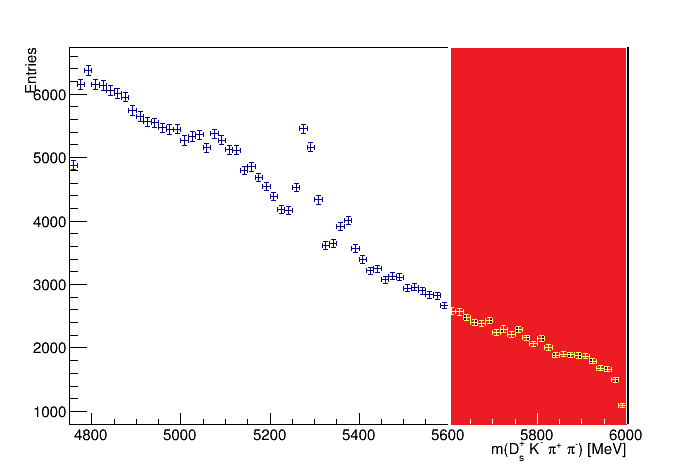
\includegraphics[height=7.4cm,width=0.7\textwidth]{figs/mass_Bs_forBDT_12_AnA.png}
%\vspace*{-0.2cm}
\caption{Invariant mass distribution of preselected $\Bs\to\Ds\kaon\pion\pion$ candidates. The red coloured region with $m_{\Bs candidate}$ $>$ 5600 $\mevcc$ is used as background input for the boosted decision tree.}
\label{fig:massforBDT}
\end{figure}

The distributions of the input variables for signal and background are shown in Fig. \ref{fig:BDT_Input_1}. 

\begin{figure}[h]
%\vspace*{-0.4cm}
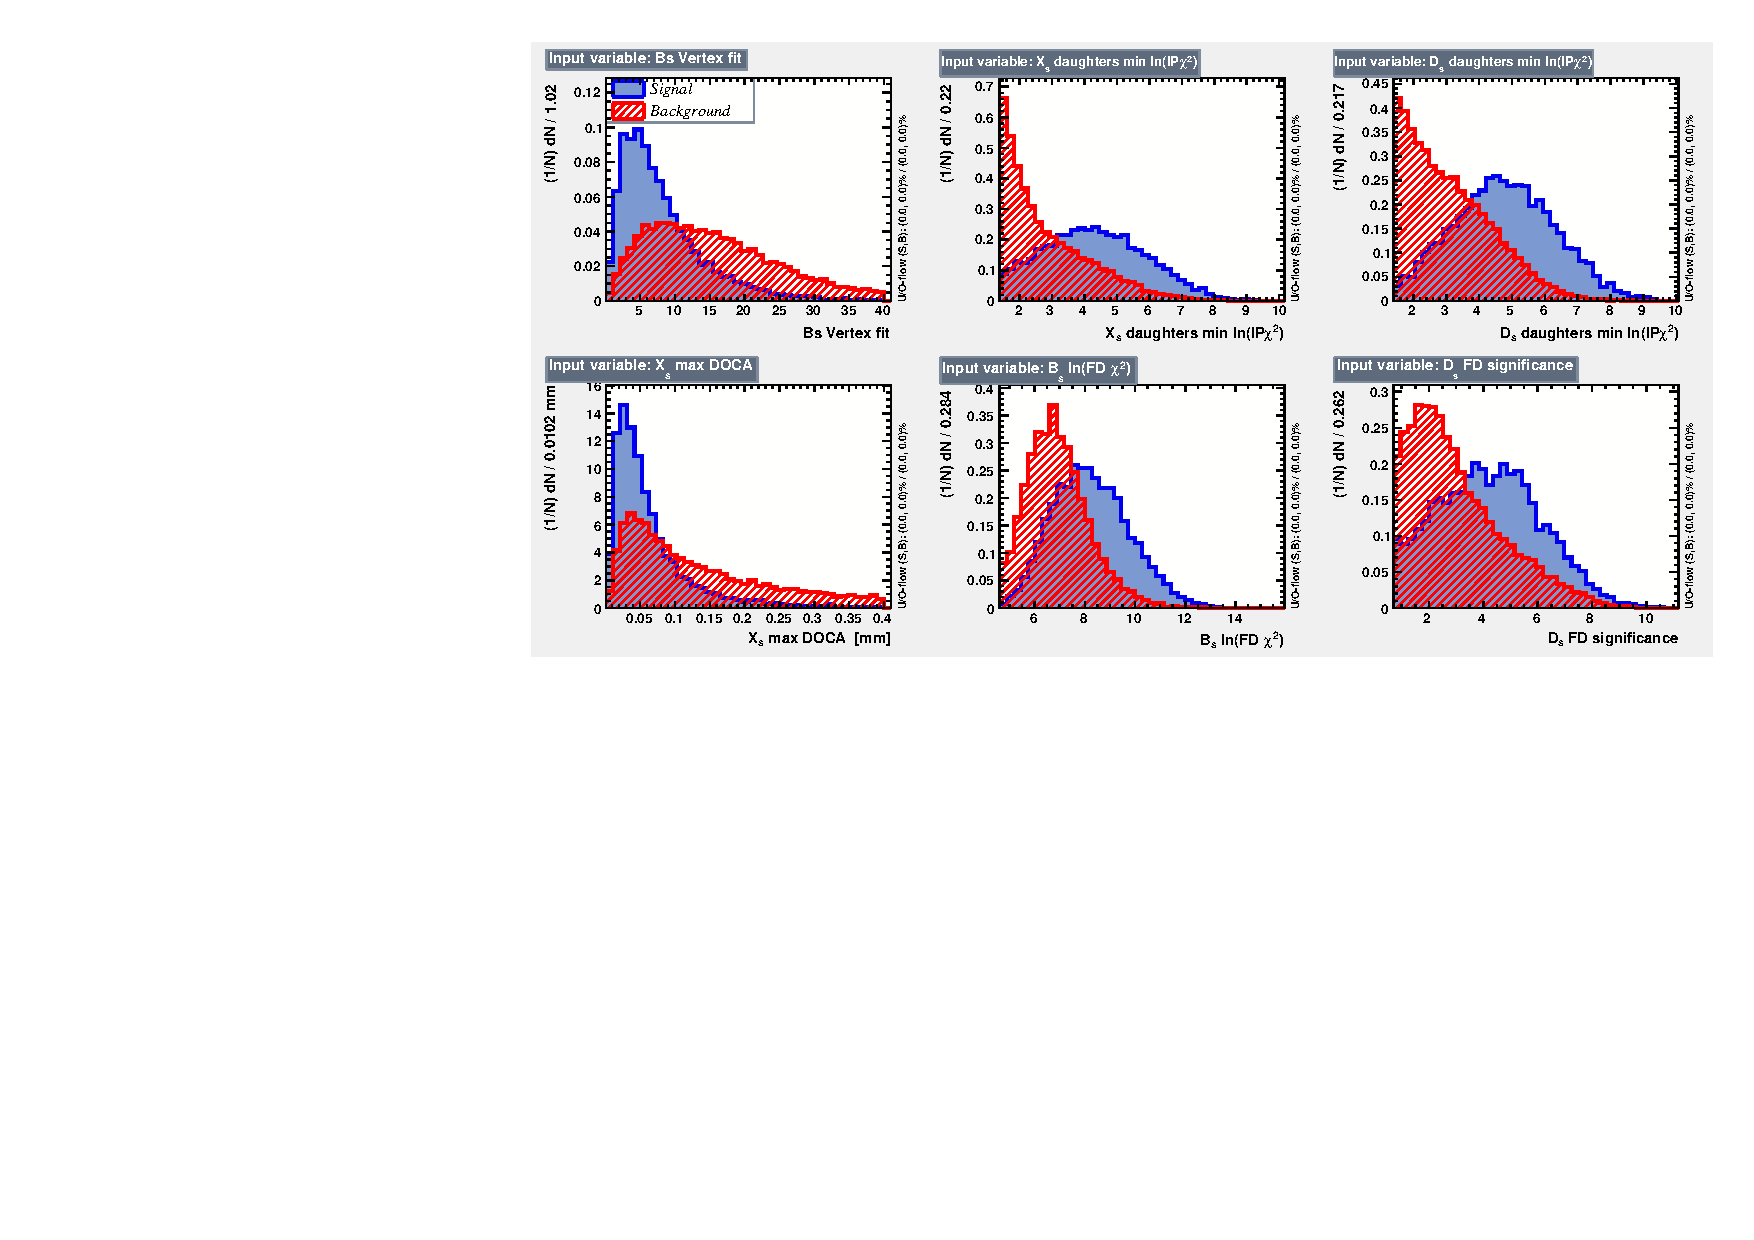
\includegraphics[height=6.cm,width=0.95\textwidth]{figs/BDT_Input_1.pdf}
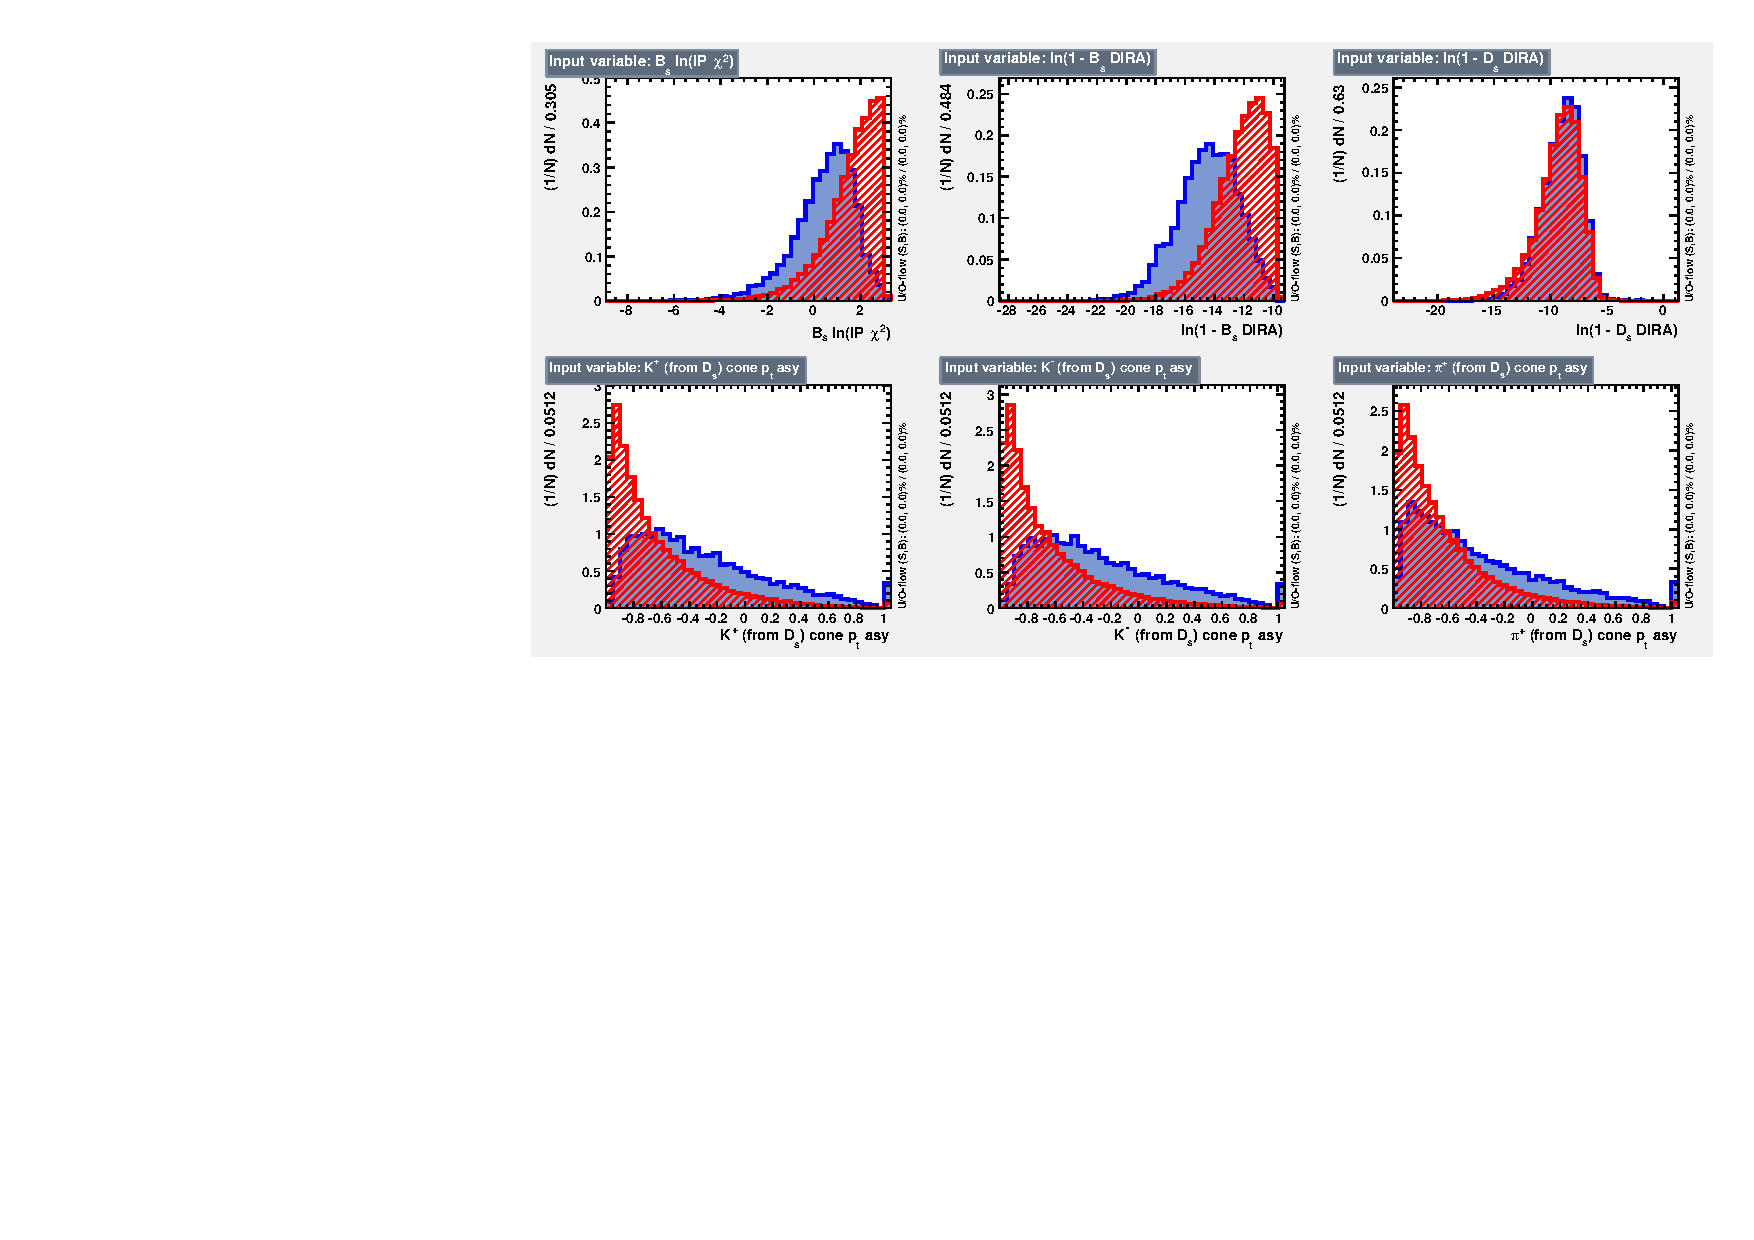
\includegraphics[height=6.cm,width=0.95\textwidth]{figs/BDT_Input_2.pdf}
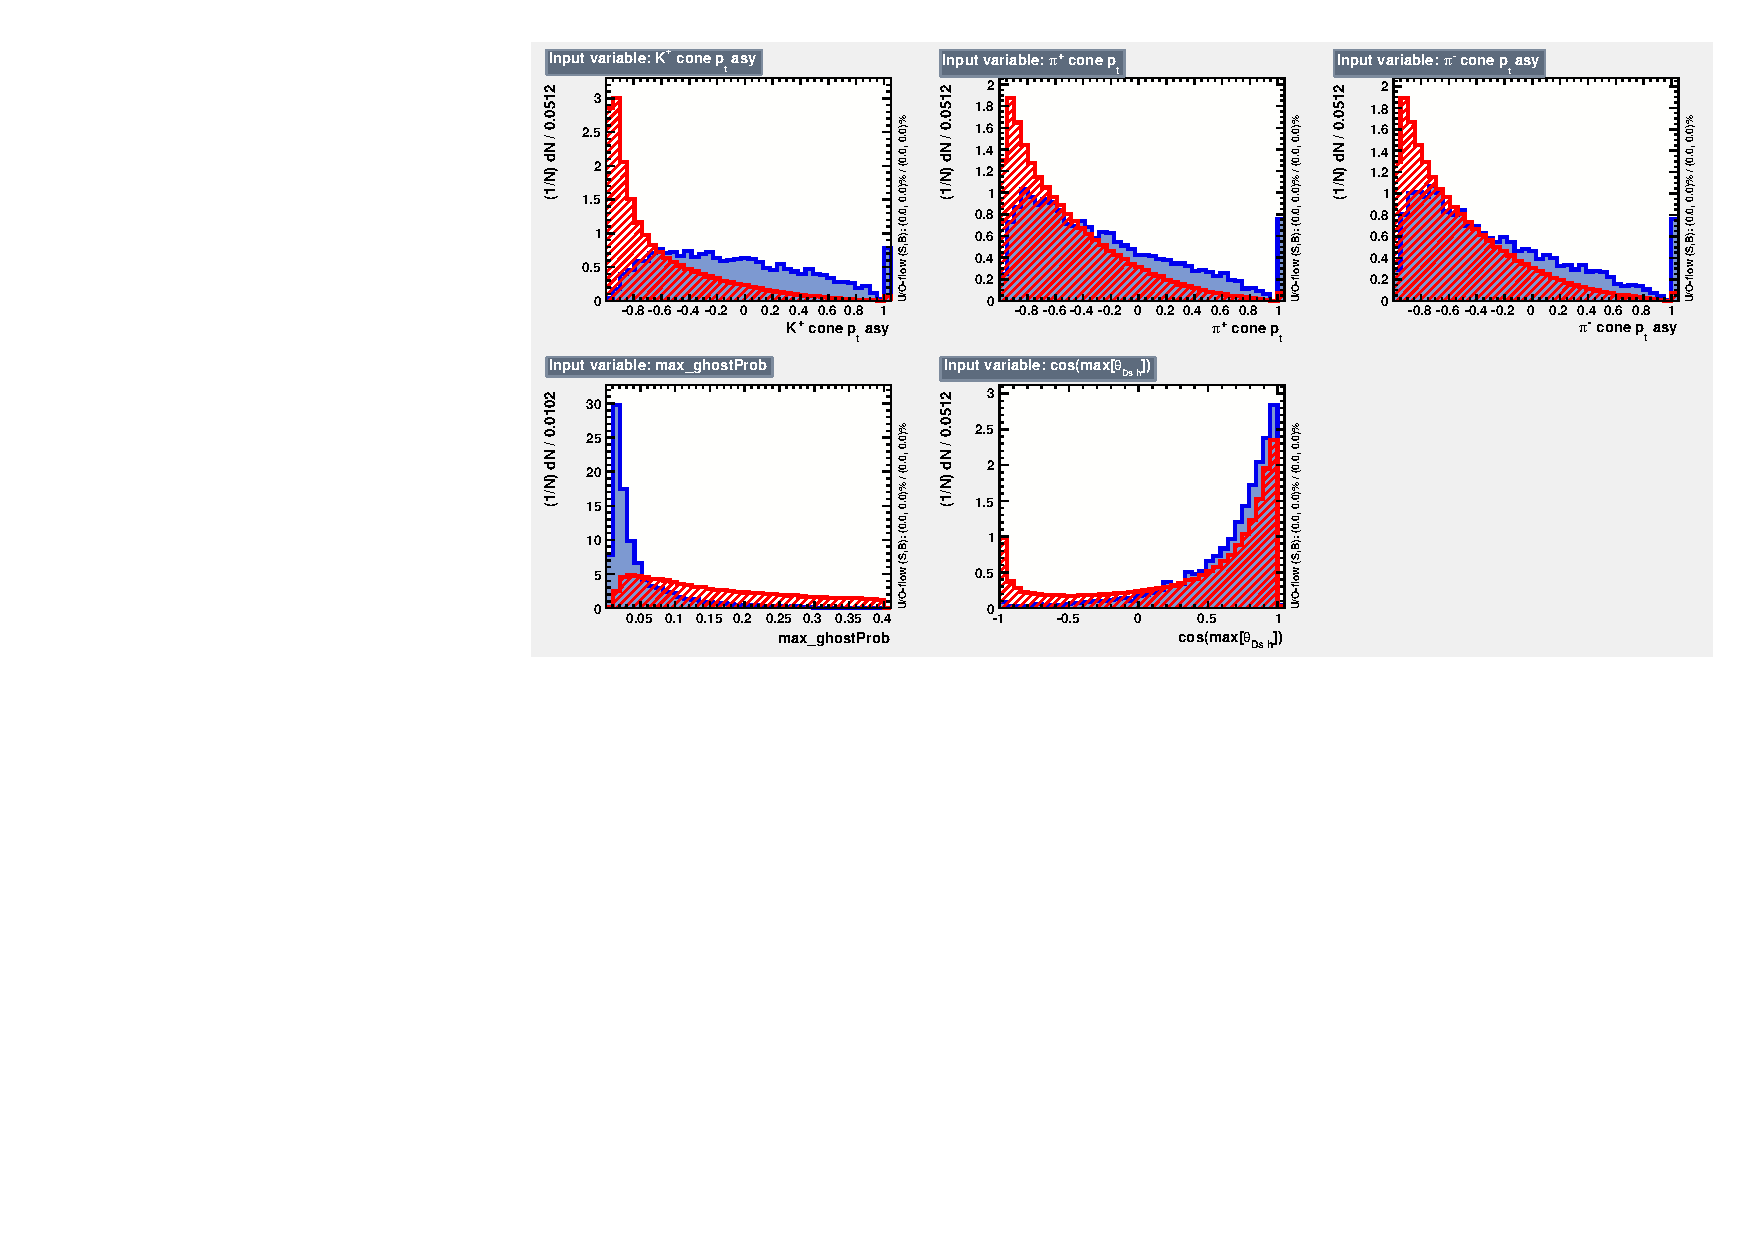
\includegraphics[height=6.cm,width=0.95\textwidth]{figs/BDT_Input_3.pdf}
%\vspace*{-0.2cm}
\caption{Distributions of the input variables used in the BDTG training. The background is shown as red hatched, while the signal is depicted solid blue.}
\label{fig:BDT_Input_1}
\end{figure}


The relative importance of the input variables for the BDTG training is summarized in Table \ref{table:InputVars}.

\begin{table}[h]
\centering
 \begin{tabular}{l c}
Variable & relative importance [$\%$]\\
  \hline
pi\_minus\_ptasy\_1.00 & 7.32\\
log\_Ds\_FDCHI2\_ORIVX & 7.23\\
K\_plus\_ptasy\_1.00 & 7.17\\
log\_Ds\_DIRA & 6.96\\
Bs\_ENDVERTEX\_CHI2 & 6.82\\
max\_ghostProb & 6.76\\
pi\_plus\_ptasy\_1.00 & 6.57\\
log\_DsDaughters\_min\_IPCHI2 & 6.21\\
log\_Bs\_DIRA & 6.15\\
K\_plus\_fromDs\_ptasy\_1.00 & 6.10\\
log\_XsDaughters\_min\_IPCHI2 & 5.87\\
K\_minus\_fromDs\_ptasy\_1.00 & 5.62\\
cos(Ds h) & 5.58\\
log\_Bs\_IPCHI2\_OWNPV & 5.08\\
log\_Bs\_FDCHI2\_OWNPV & 4.04\\
Xs\_max\_DOCA & 3.98\\
pi\_minus\_fromDs\_ptasy\_1.00 & 2.59\\
\end{tabular}
\caption{Summary of the relative importance of each variable in the training of the BDTG.}
\label{table:InputVars}
\end{table}

 
The BDTG output distribution for test and training samples is shown in Fig \ref{fig:BDT_Response}. No sign of overtraining is observed. 

\begin{figure}[h]
%\vspace*{-0.4cm}
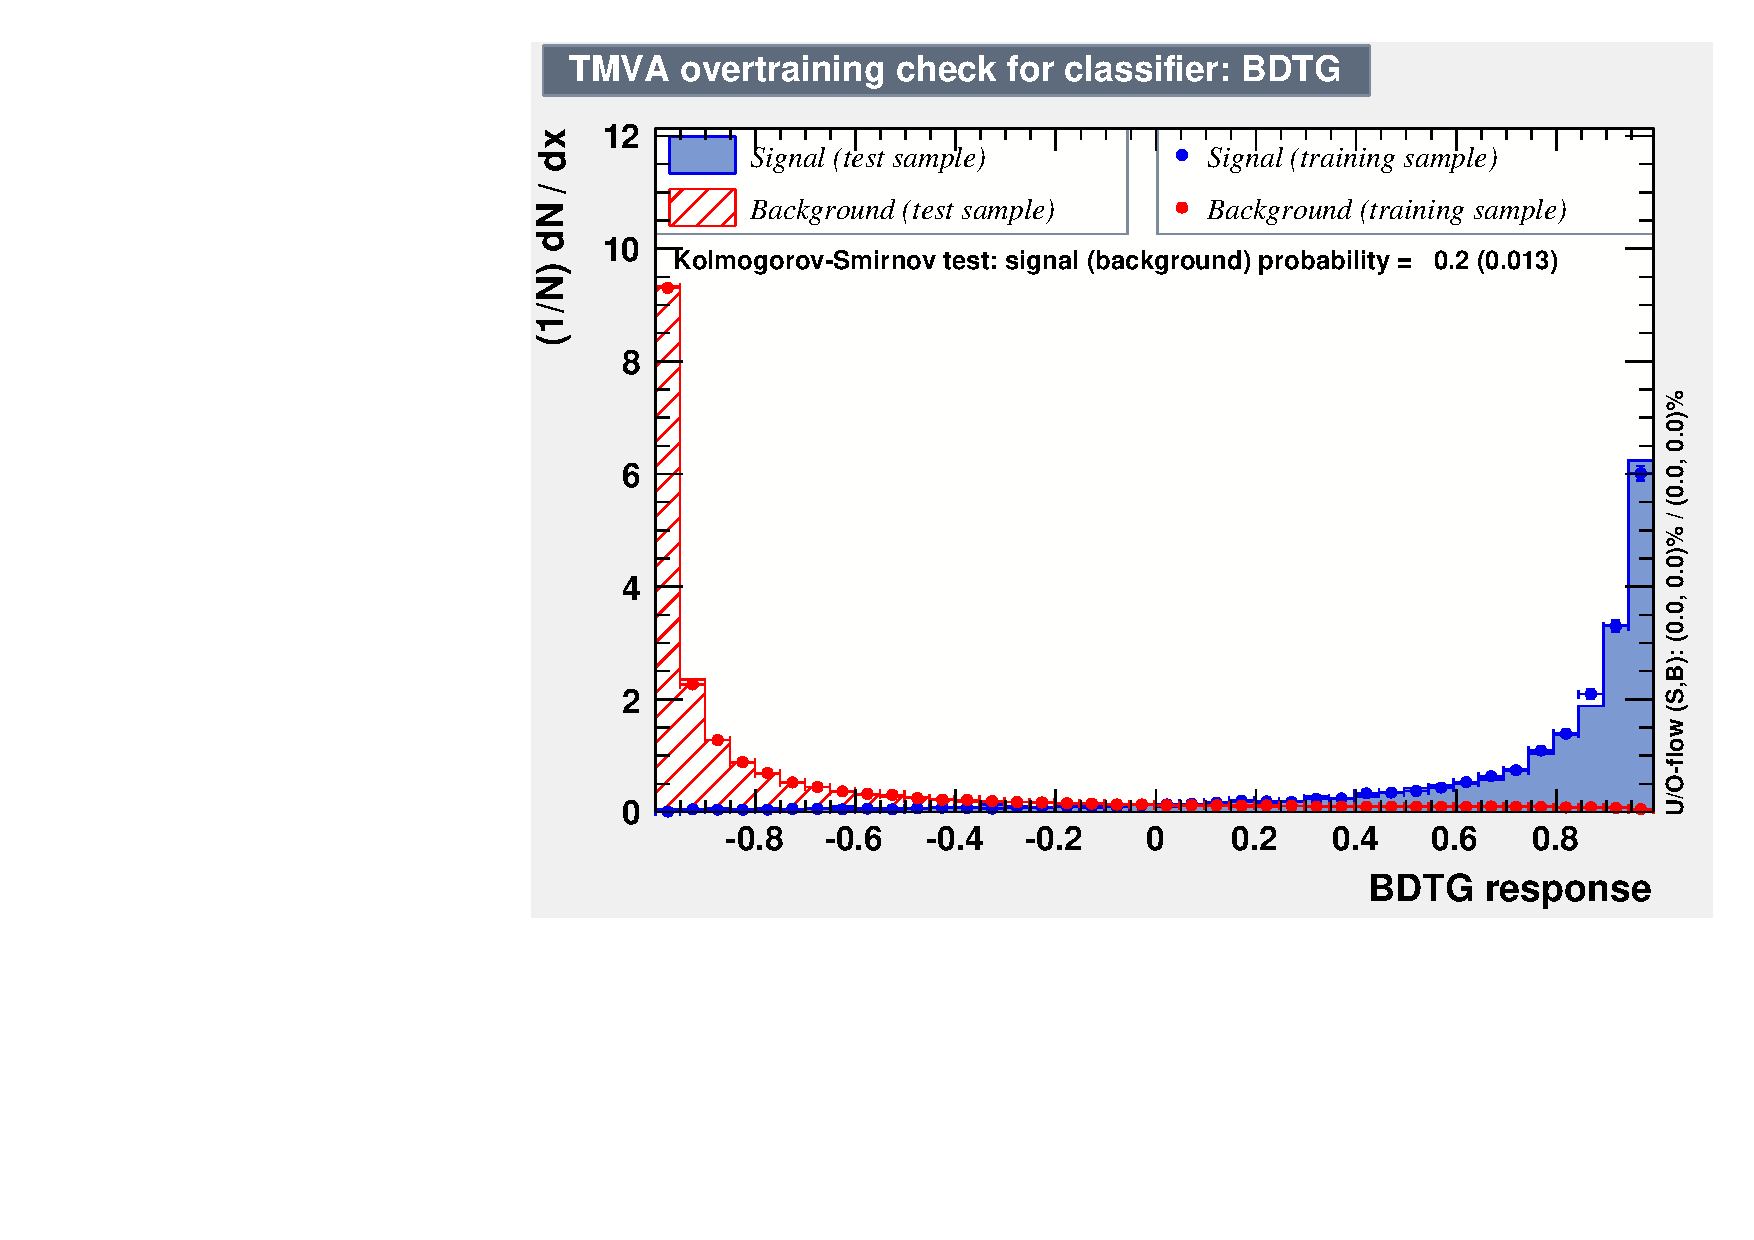
\includegraphics[height=7.4cm,width=0.7\textwidth]{figs/BDT_Response_new.pdf}
%\vspace*{-0.2cm}
\caption{BDTG output classifier distribution for (blue) signal and (red) background. The response of an independent test sample (dots) is overlaid.}
\label{fig:BDT_Response}
\end{figure}


       
We determine the optimal cut value by maximizing the figure of merit $S/\sqrt{S+B}$ where S is the signal yield and B the background yield in the signal region, defined to be within $\pm$50 $\mevcc$ of the nominal $\Bs$ mass. 
To avoid a bias in the determination of the branching fraction, we determine S and B using our normalization channel. 
All trigger, stripping and additional selection criteria described in this and the previous chapter are applied to the $\Bs\to\Ds\pion\pion\pion$ data samples. 
After that, we perform a simplified version of the fit to the invariant mass distribution of $\Bs\to\Ds\pion\pion\pion$ candidates described in Sec.~\ref{sec: fitting}.
Here, a Gaussian function to model the signal and an exponential function to model combinatorial background is used.
From this fit we estimate the number of signal events in our normalization channel. 
Multiplying that number with the PDG branching fraction of $\frac{\mathcal{B}(\Bs\to\Ds\kaon\pion\pion)}{\mathcal{B}(\Bs\to\Ds\pion\pion\pion)}$ and the ratio of efficiencies discussed in Sec. \ref{sec: efficiency} allows us to estimate the expected number of $\Bs\to\Ds\kaon\pion\pion$ signal decays. The number of background events can then be computed as

\begin{equation}
 N_{bkg}=N_{all}-N_{sig}|_{m_{\Bs\pm50\mevcc}}.   
\end{equation}

The efficiency curves as a function of the cut value are shown in Fig. \ref{fig:BDT_Efficiency}. 
The optimal cut value is found to be BDTG $>$ 0.7012. At this working point the signal efficiency is estimated to be 72.47 $\%$, while the background rejection in the signal region is 97.38 $\%$. 


\begin{figure}[h]
%\vspace*{-0.4cm}
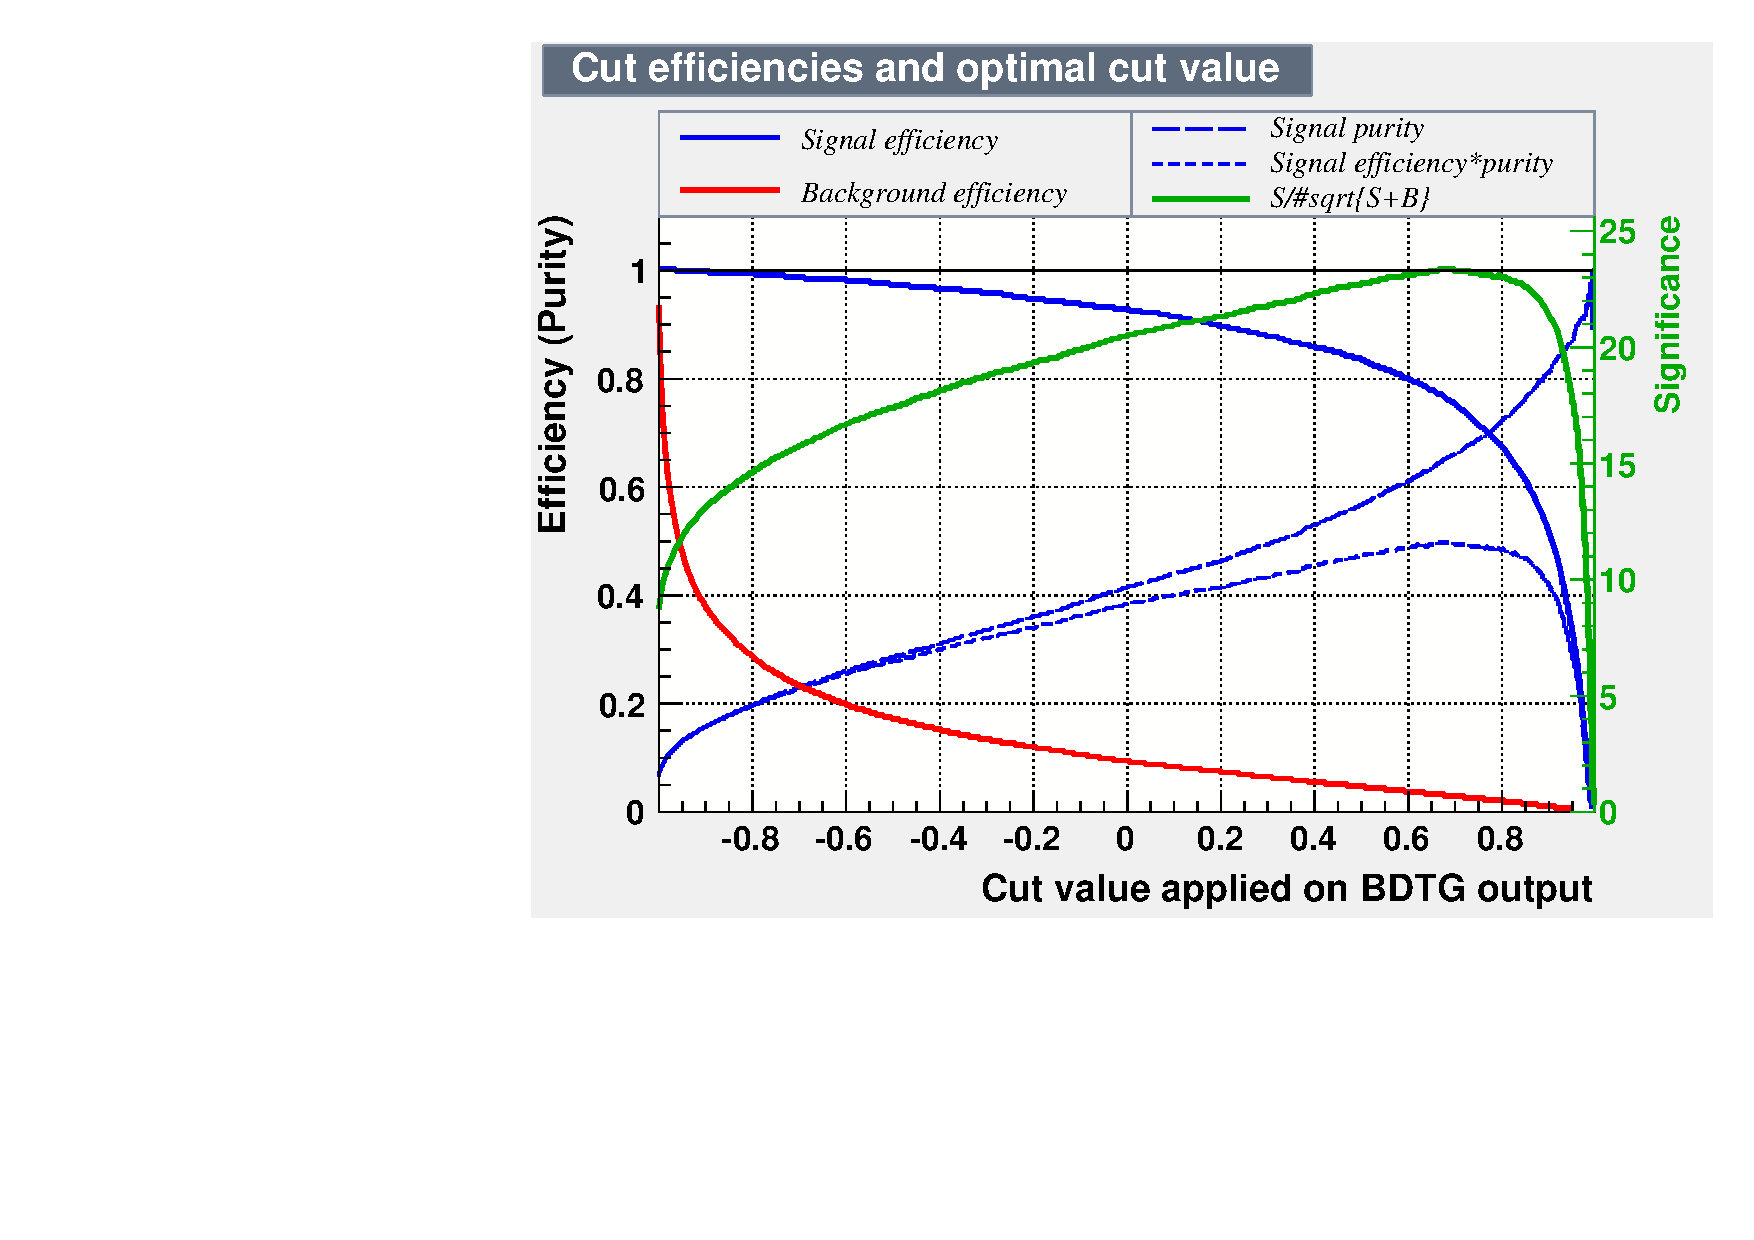
\includegraphics[height=7.4cm,width=0.7\textwidth]{figs/BDT_CutEfficiency.pdf}
%\vspace*{-0.2cm}
\caption{Efficiency and purity curves for (blue) signal, (red) background and the (green) FoM curve, as a function of the chosen cut value.}
\label{fig:BDT_Efficiency}
\end{figure}
